\chapter{描述化学体系：反应进度、活度、Q 与 K}\label{ch:b1:extent-q-and-k}

制氢厂将天然气与水蒸气送入烧至炽热的管中，
流出的并非纯氢，而是氢气、一氧化碳、二氧化碳、
未反应的甲烷与水蒸气的混合物，其比例须由工程师
在设计下一单元之前掌握。预测反应器出口的组成，
即化学体系的最终状态，是本章的主题。
这需要对体系作精确的描述（包括其变量与组成），
需要一个衡量反应进行程度的量（反应进度），
还需要一条规律来说明反应在何处停止，
即平衡常数。
这些工具在此后关于溶液的各章中都会用到。

\begin{recall}
第 1 册（十年级）用进度表跟踪反应，
求出限量反应物；第 1 册（十二年级）引入了非完全反应的反应商
$Q$ 与平衡常数 $K$。从物理学中可用理想气体定律
$pV = nRT$，其中 $R =
\qty{8.314}{J/(mol.K)}$。
\end{recall}

\begin{omfigure}
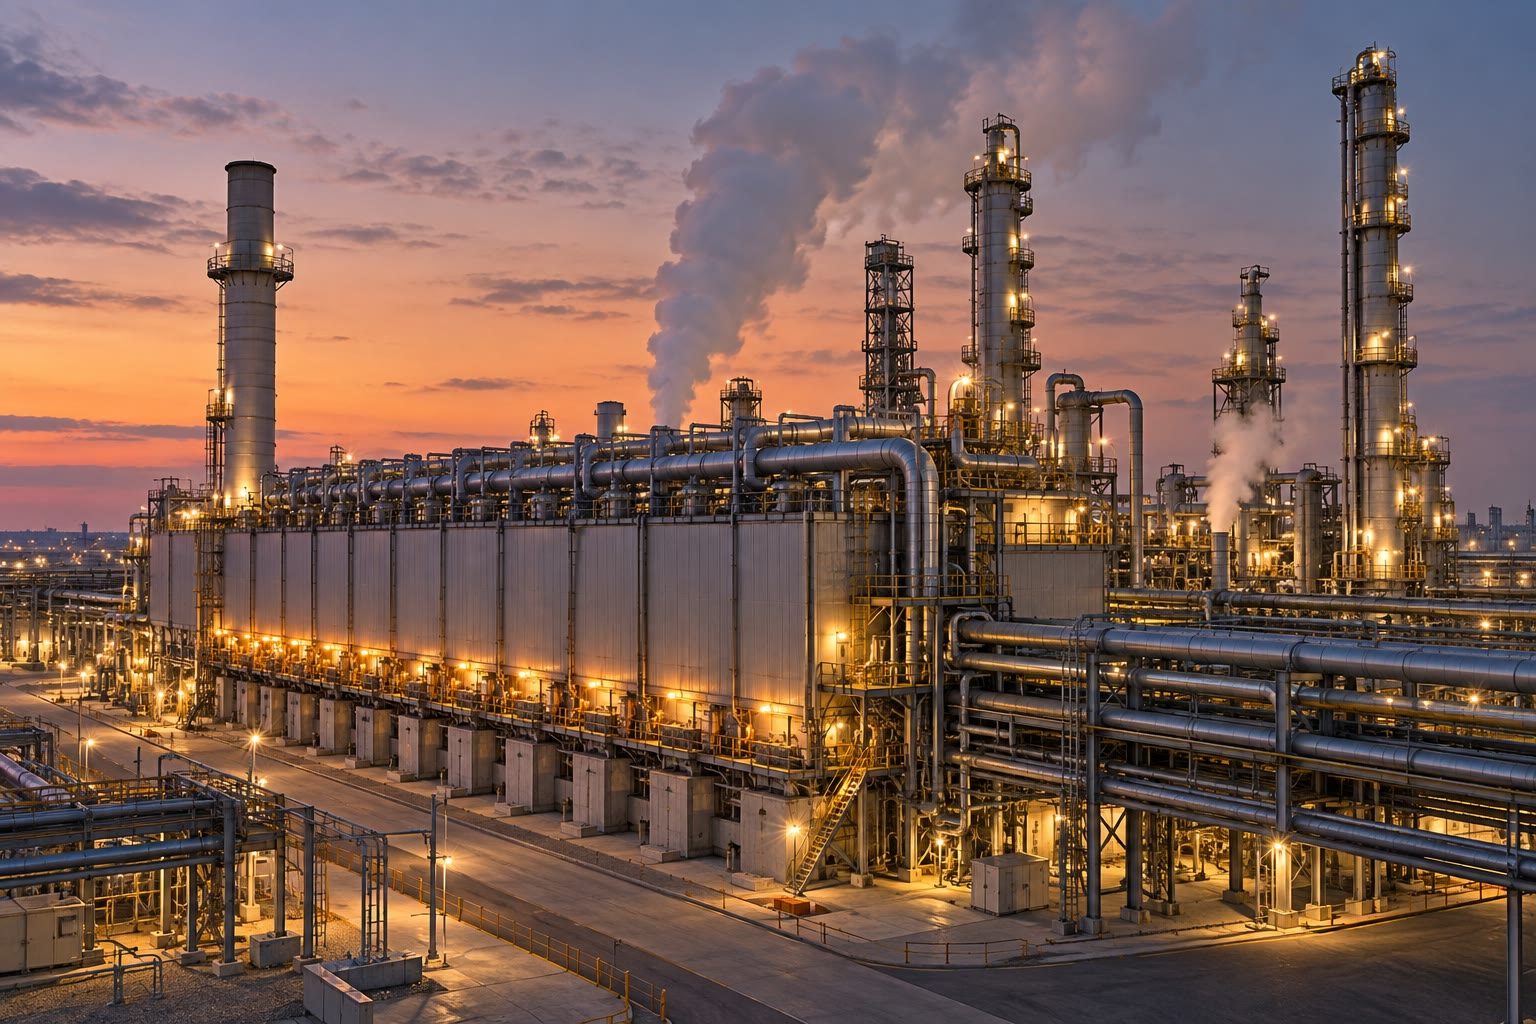
\includegraphics[width=0.6\linewidth]{images/book2/ai/b1-07-hydrogen-plant.jpg}

{\small 黄昏时分的制氢厂。天然气与水蒸气
在长型重整炉中发生反应；第二个反应器
转化一氧化碳；出口组成
即为本章所计算的那类最终状态。}
\end{omfigure}

\section{描述体系}

\begin{definition}[体系，相]\label{def:b1:extent-q-and-k:system}
\emph{物理化学体系}\index{物理化学体系}是指所选空间区域内所含的
物质，区域之外称为其外界。
若体系与外界不交换物质，则称其为
\emph{封闭体系}\index{封闭体系}（可以交换能量）。
体系中强度量连续变化的一部分称为一个
\emph{相}\index{相}：气体混合物为一个相，两种不互溶的液体为两个相，
每一块固体各自为一个相。
\end{definition}

\begin{definition}[强度量与广延量]\label{def:b1:extent-q-and-k:variables}
状态变量若与体系的大小成正比（如质量、体积、物质的量），
则称其为\emph{广延量}\index{广延量}；
若不成正比（如温度、压强、浓度、密度、摩尔分数），
则称其为\emph{强度量}\index{强度量}。
两个广延量之比为强度量。
\end{definition}

\begin{definition}[组成变量]\label{def:b1:extent-q-and-k:composition}
对某相中的组分 $i$，设该相含有其全部组分的物质的量 $n_j$，
则有：
\begin{itemize}
  \item 其\emph{摩尔分数}\index{摩尔分数}为 $x_i = n_i/\sum_j
        n_j$，\emph{质量分数}\index{质量分数} $w_i =
        m_i/\sum_j m_j$；二者均介于 0 与 1 之间，且和为 1；
  \item 在体积为 $V$ 的溶液中，其
        \emph{物质的量浓度}\index{物质的量浓度}为 $c_i = [i] = n_i/V$，
        单位为 \unit{mol/L}；
  \item 在总压为 $p$ 的气体混合物中，其\emph{分压}\index{分压}
        为 $p_i = x_i\,p$。
\end{itemize}
\end{definition}

\begin{proposition}[理想气体的分压]\label{prop:b1:extent-q-and-k:dalton}
在体积为 $V$、温度为 $T$ 的理想气体混合物中，
某组分的分压是该组分单独占据整个体积时
所产生的压强，即 $p_i = n_iRT/V$，且各分压之和
等于总压：$\sum_i p_i = p$。
\end{proposition}

\begin{proof}
对于混合物有 $pV = (\sum_j n_j)RT$，故 $p_i = x_i p = \frac{n_i}{\sum_j
n_j}\cdot\frac{(\sum_j n_j)RT}{V} = \frac{n_iRT}{V}$；由 $\sum_i x_i = 1$
得 $\sum_i p_i = p$。
\end{proof}

\begin{example}[空气]\label{ex:b1:extent-q-and-k:air}
干燥空气按体积计（对理想气体即按物质的量计），
含氮气 78.08\,\%、氧气 20.95\,\% 和氩气 0.93\,\%。在 \qty{1.013}{bar} 下，
氧气的分压为 $0.2095 \times
1.013 = \qty{0.212}{bar}$；在压强为
\qty{0.70}{bar} 的山上，其分压降至 \qty{0.147}{bar}，
尽管组成并未改变。
% ledger: air:N2, air:O2, air:Ar, const:atm
\end{example}

\section{反应进度}

\begin{definition}[化学计量数与反应进度]\label{def:b1:extent-q-and-k:extent}
反应写作 $0 = \sum_i \nu_i\,\mathrm{A}_i$，其中
\emph{化学计量数}\index{化学计量数} $\nu_i$ 对物种 $\mathrm{A}_i$ 而言，
反应物取负、生成物取正，例如在
\ce{N2 + 3H2 -> 2NH3} 中，$\nu(\ce{N2}) = -1$，$\nu(\ce{H2}) = -3$，
$\nu(\ce{NH3}) = +2$。
若封闭体系中只发生该反应，则各物质的量按下式变化：
\[
  n_i = n_{i,0} + \nu_i\,\xi ,
\]
由此定义\emph{反应进度}\index{反应进度}
$\xi$（单位为摩尔），其初始值为零，且对每种物质都相同。
\end{definition}

\begin{definition}[最大反应进度，限量反应物]\label{def:b1:extent-q-and-k:max-extent}
\emph{最大反应进度}\index{最大反应进度} $\xi_{\max}$ 是使各物质的量都不为负的
$\xi$ 的最大值：$\xi_{\max} = \min_{\nu_i <
0} n_{i,0}/|\nu_i|$。在 $\xi_{\max}$ 时降为零的反应物为
\emph{限量反应物}\index{限量反应物}。若反应进度也可为负（即逆反应），
则 $\xi_{\min} = -\min_{\nu_i > 0}
n_{i,0}/\nu_i$。
\end{definition}

\begin{method}[进度表]\label{met:b1:extent-q-and-k:progress-table}
对封闭系统中的反应进行跟踪：
\begin{enumerate}
  \item 写出配平的方程式，并在其下为每种物质设一列；
  \item 第一行：初始物质的量 $n_{i,0}$；
  \item 第二行：反应进度为 $\xi$ 时的物质的量 $n_{i,0} + \nu_i\xi$；
  \item 对于气体，增加一列，表示总物质的量 $n_{\text{总}}(\xi)$；
  \item 计算 $\xi_{\max}$（及 $\xi_{\min}$），并确定限量
        反应物；
  \item 最后一行：最终物质的量，对应最终反应进度 $\xi_f$（由平衡条件
        求得，或在反应完全时
        等于 $\xi_{\max}$）。
\end{enumerate}
\end{method}

\begin{example}[合成氨]\label{ex:b1:extent-q-and-k:ammonia}
以 \qty{2.0}{mol} 的 \ce{N2} 与 \qty{3.0}{mol} 的 \ce{H2} 为原料：
\begin{center}
\begin{tabular}{lcccc}
\hline
 & \ce{N2} & \ce{3H2} & \ce{2NH3} & 总计 \\
\hline
初始 & 2.0 & 3.0 & 0 & 5.0 \\
反应进度 $\xi$ & $2.0 - \xi$ & $3.0 - 3\xi$ & $2\xi$ & $5.0 - 2\xi$ \\
\hline
\end{tabular}
\end{center}
$\xi_{\max} = \min(2.0/1,\ 3.0/3) = \qty{1.0}{mol}$：限量反应物为氢气。
若反应为完全反应，则最终状态中含 \qty{1.0}{mol}
\ce{N2} 与 \qty{2.0}{mol} \ce{NH3}。
\end{example}

\begin{definition}[最终转化率，产率]\label{def:b1:extent-q-and-k:fractional-extent}
某反应的\emph{最终转化率}\index{最终转化率}
为 $\tau = \xi_f/\xi_{\max}$，取值介于 0 与 1 之间。在合成反应中，某产物的
\emph{产率}\index{产率}是所得该产物的物质的量
与限量反应物在反应完全时可得的该产物物质的量之比；
若分离过程中产物没有损失，则产率等于 $\tau$。
\end{definition}

\section{活度}

\begin{definition}[标准态，活度]\label{def:b1:extent-q-and-k:activity}
某物种的\emph{活度}\index{活度} $a_i$ 是一个无量纲的
数，用来度量其在平衡定律表达式中有多少可供利用；
它是相对于\emph{标准
态}\index{标准态}定义的，即在所考虑的温度下的参考状态，
并以标准压强 $p^\circ = \qty{1}{bar}$ 为基准。在本书采用的
理想近似下：
\begin{itemize}
  \item 对于气体，$a_i = p_i/p^\circ$（标准态为
        $p^\circ$ 下的纯理想气体）；
  \item 对于稀溶液中的溶质，$a_i = c_i/c^\circ$，其中
        $c^\circ = \qty{1}{mol/L}$；
  \item 对于稀溶液中的溶剂，以及单独处于其相中的纯固体或
        纯液体，$a_i = 1$。
\end{itemize}
\end{definition}
% ledger: const:pstd

\begin{remark}[理想与实际]\label{rem:b1:extent-q-and-k:ideal}
这些表达式适用于理想气体与稀溶液。在浓溶液中，
离子之间相互吸引与排斥，活度偏离 $c_i/c^\circ$；
其修正以活度系数表示，
相关内容在本科二年级分册中结合化学势加以研究。
对于本书所用的浓度（约低于
\qty{0.1}{mol/L}）时，理想表达式的误差在百分之几以内。
\end{remark}

\section{反应商与平衡常数}

\begin{definition}[反应商]\label{def:b1:extent-q-and-k:quotient}
在体系的给定状态下，反应的\emph{反应商}\index{反应商}
（对于 $0 = \sum_i \nu_i\,\mathrm{A}_i$）为
\[
  Q = \prod_i a_i^{\nu_i} ,
\]
即各生成物活度之积除以各反应物活度之积，
每项均取其化学计量数为指数。
\end{definition}

\begin{example}[三个反应商]\label{ex:b1:extent-q-and-k:quotients}
对于 \ce{N2(g) + 3H2(g) <=> 2NH3(g)}：$Q = \dfrac{(p_{\ce{NH3}}/p^\circ)^2}
{(p_{\ce{N2}}/p^\circ)(p_{\ce{H2}}/p^\circ)^3}$。对于
\ce{CH3COOH(aq) + H2O(l) <=> CH3COO^-(aq) + H3O+(aq)}：$Q =
\dfrac{[\ce{CH3COO-}][\ce{H3O+}]}{[\ce{CH3COOH}]\,c^\circ}$，其中溶剂
活度为 1。对于 \ce{CaCO3(s) <=> CaO(s) + CO2(g)}：$Q =
p_{\ce{CO2}}/p^\circ$，其中固体活度均为 1。
\end{example}

\begin{definition}[标准平衡常数]\label{def:b1:extent-q-and-k:equilibrium-constant}
反应的\emph{标准平衡常数}\index{标准平衡常数}
$K^\circ$ 是体系达到平衡时其反应商所取的值。
它是无量纲的，
且仅依赖于反应与温度。
\end{definition}

\begin{theorem}[质量作用定律]\label{thm:b1:extent-q-and-k:mass-action}
在给定温度下，若反应可在两个方向上进行，
则体系将演化至 $Q = K^\circ(T)$；平衡时，
无论初始组成如何，
\[
  \prod_i a_{i,\text{平衡}}^{\nu_i} = K^\circ(T) .
\]
\end{theorem}
\admitted

\begin{proposition}[演化方向]\label{prop:b1:extent-q-and-k:direction}
若 $Q < K^\circ$，体系向正方向演化（$\xi$
增大）；若 $Q > K^\circ$，则向逆方向演化；若
$Q = K^\circ$，则体系处于平衡状态。
\end{proposition}
\admitted

\begin{remark}[这些定律的来源]\label{rem:b1:extent-q-and-k:origin}
两条陈述均由热力学第二定律导出，通过
反应的自由能与各物种的化学势：它们
在本科二年级分册中推导，该分册还由热力学数据表给出 $K^\circ$，
并说明其如何随温度变化。此处
将它们作为定律使用。
\end{remark}

\begin{omfigure}
\begin{tikzpicture}[font=\small, >={Stealth}]
  \draw[->, thick] (0,0) -- (11,0) node[right] {$Q$};
  \draw[thick, omThm] (5.5,0.25) -- (5.5,-0.25) node[below] {$K^\circ$};
  \draw[->, omDef, thick] (1.0,0.55) -- (4.6,0.55);
  \node[above, omDef] at (2.8,0.6) {$Q < K^\circ$：正向};
  \draw[->, omProp, thick] (10.0,0.55) -- (6.4,0.55);
  \node[above, omProp] at (8.2,0.6) {$Q > K^\circ$：逆向};
  \node[below] at (0,-0.1) {0};
\end{tikzpicture}

{\small 商向平衡常数靠拢：$Q <
K^\circ$ 的体系生成产物，$Q > K^\circ$ 的体系则消耗产物。}
\end{omfigure}

\begin{proposition}[平衡常数的组合]\label{prop:b1:extent-q-and-k:combine-k}
若 $K_1^\circ$ 与 $K_2^\circ$ 分别为反应（1）与（2）的平衡常数：
反应（1）的逆反应平衡常数为 $1/K_1^\circ$；反应 $n \times
(1)$ 的平衡常数为 $(K_1^\circ)^n$；和反应 $(1) + (2)$ 的平衡常数为 $K_1^\circ K_2^\circ$。
\end{proposition}

\begin{proof}
逆反应的商为 $\prod a_i^{-\nu_i} = 1/Q_1$；
$n \times (1)$ 的商为 $\prod a_i^{n\nu_i} = Q_1^n$；和的商为
$\prod a_i^{\nu_{i,1} + \nu_{i,2}} = Q_1 Q_2$。将这些恒等式写在
平衡时（此时各商都等于其平衡常数），即得结论。
\end{proof}

\begin{proposition}[唯一平衡状态]\label{prop:b1:extent-q-and-k:q-monotone}
对封闭系统中的单一反应，在温度固定时（对气体，
体积或压强也固定），商 $Q(\xi)$ 是
关于 $\xi$ 的严格递增函数，在 $(\xi_{\min}, \xi_{\max})$ 上从 0
增至 $+\infty$（不涉及活度恒定的物种时）。
方程 $Q(\xi) = K^\circ$ 于是在此
区间内恰有一个解。
\end{proposition}

\begin{proof}
考虑溶液中的反应，$Q(\xi) = \prod_i (n_{i,0} + \nu_i\xi)^{\nu_i}
\times \text{常数}$。其对数导数为
\[
  \frac{\dd \ln Q}{\dd \xi} = \sum_i \frac{\nu_i^2}{n_{i,0} + \nu_i \xi}
  > 0 ,
\]
各项在所有物质的量均为正时为正。当 $\xi \to \xi_{\max}$ 时，一种
反应物的量在分母中趋于 0，$Q \to +\infty$；当 $\xi
\to \xi_{\min}$ 时，一种生成物的量趋于 0，$Q \to 0$。一个连续
递增函数从 0 增至 $+\infty$，恰好一次取值 $K^\circ$。
（对恒压下的气体，总物质的量也会变化；结论
仍成立，可逐一验证。）
\end{proof}

\section{最终状态}

\begin{definition}[平衡状态，定量反应]\label{def:b1:extent-q-and-k:quantitative}
最终状态称为\emph{平衡状态}\index{平衡状态}，
即反应中所有物种均存在且 $Q = K^\circ$。反应
称为\emph{定量反应}\index{定量反应}（即完全反应），
即在最终状态下，限量反应物
几乎耗尽，$\xi_f \approx \xi_{\max}$；这发生于 $K^\circ$
很大时。
\end{definition}

\begin{method}[求最终状态]\label{met:b1:extent-q-and-k:final-state}
求单一反应的最终状态，步骤为：
\begin{enumerate}
  \item 画出进度表，计算 $\xi_{\max}$（及 $\xi_{\min}$）；
  \item 计算起始时的 $Q$，并与 $K^\circ$ 比较，以确定
        方向；
  \item 用活度表示 $Q(\xi)$，并解方程 $Q(\xi) = K^\circ$
        求 $\xi$，其位于 $(\xi_{\min}, \xi_{\max})$ 内；
  \item 若涉及活度为 1 的物种（固体），须检查该物种在此反应进度下
        仍然存在：若其量须变为负值，
        则它先被耗尽，终态\emph{不是}
        平衡状态（$\xi_f = \xi_{\max}$，$Q_f \ne K^\circ$）。
\end{enumerate}
\end{method}

\begin{method}[定量反应假设]\label{met:b1:extent-q-and-k:quantitative}
当 $K^\circ$ 较大（通常大于 $10^4$）时，假设反应
完全进行：取 $\xi_f = \xi_{\max}$，计算终态各物质的量，再求
限量反应物剩余的少量 $\varepsilon$，即写出 $Q =
K^\circ$，其他物质的量保持不变。若
$\varepsilon$ 与其他物质的量相比很小（约低于
1\,\%），则该假设成立。
\end{method}

\begin{example}[定量反应]\label{ex:b1:extent-q-and-k:quant}
对溶液中的 $\mathrm{A + B \rightleftharpoons C + D}$，取 $[\ce{A}]_0 = [\ce{B}]_0 =
\qty{0.10}{mol/L}$，且 $K^\circ = 10^6$：假设完全反应，$[\ce{C}]
= [\ce{D}] = 0.10$；由 $0.10^2/\varepsilon^2 = 10^6$ 得 $\varepsilon
= \qty{1.0e-4}{mol/L}$，为初始量的 0.1\,\%，该假设
是合理的。
\end{example}

\begin{omfigure}
\begin{tikzpicture}
\begin{axis}[
  width=0.45\linewidth, height=5.6cm, ymode=log,
  xmin=0, xmax=1, ymin=0.01, ymax=1000,
  axis x line=bottom, axis y line=left,
  xlabel={反应进度 $\xi$（mol）}, ylabel={$Q$}, xtick={0,0.2,0.4,0.8,1},
  tick label style={font=\small}, label style={font=\small}, clip=false]
\addplot[omDef, thick] table[x=xi, y=Q] {figdata/out/bachelor-1-extent-equilibrium-shift.dat};
\draw[omThm, dashed] (axis cs:0,4) -- (axis cs:1,4);
\node[omThm, anchor=south west, font=\small] at (axis cs:0.02,4) {$K^\circ = 4.0$};
\draw[dotted] (axis cs:0.607,0.01) -- (axis cs:0.607,4);
\node[anchor=north, font=\small] at (axis cs:0.607,0.01) {0.607};
\end{axis}
\end{tikzpicture}\hfill
\begin{tikzpicture}
\begin{axis}[
  width=0.45\linewidth, height=5.6cm,
  xmin=0, xmax=0.04, ymin=0, ymax=0.3,
  axis x line=bottom, axis y line=left,
  xlabel={反应进度 $\xi$（mol）}, ylabel={$Q = p_{\ce{CO2}}/p^\circ$},
  xtick={0,0.01,0.02,0.03,0.04}, scaled x ticks=false,
  xticklabel style={/pgf/number format/fixed, /pgf/number format/precision=2},
  yticklabel style={/pgf/number format/fixed},
  tick label style={font=\small}, label style={font=\small}, clip=false]
\addplot[omProp, thick] table[x=xi, y=Q_small] {figdata/out/bachelor-1-extent-equilibrium-carbonate.dat};
\addplot[omDef, thick, dashed] table[x=xi, y=Q_large] {figdata/out/bachelor-1-extent-equilibrium-carbonate.dat};
\draw[omThm, dashed] (axis cs:0,0.2) -- (axis cs:0.04,0.2);
\node[omThm, anchor=south west, font=\small] at (axis cs:0.0005,0.2) {$K^\circ = 0.20$};
 \node[omProp, anchor=north west, font=\scriptsize] at (axis cs:0.012,0.088) {\qty{0.010}{mol}：固体消失};
 \node[omDef, anchor=north west, font=\scriptsize] at (axis cs:0.024,0.19) {\qty{0.050}{mol}：平衡};
\end{axis}
\end{tikzpicture}

{\small 左：\ce{CO + H2O <=> CO2 + H2} 的反应商随
反应进度增大而上升，并与 $K^\circ$ 相交一次（周末问题）。右：对于
\ce{CaCO3(s) <=> CaO(s) + CO2(g)} 在 \qty{10}{L} 的封闭容器中，
$Q = p_{\ce{CO2}}/p^\circ$ 随 $\xi$ 增大；取 \qty{0.050}{mol} 的
碳酸钙时达到 $K^\circ = 0.20$（平衡），若取 \qty{0.010}{mol}
碳酸钙先被耗尽，终态不是
平衡态。}
\end{omfigure}

\begin{method}[两个同时发生的反应]\label{met:b1:extent-q-and-k:two-reactions}
若同一体系中同时发生两个反应，则分别给每个反应各自的
反应进度 $\xi_1$ 与 $\xi_2$；每种物质的量为 $n_i = n_{i,0} + \nu_{i,1}\xi_1
+ \nu_{i,2}\xi_2$，且终态同时满足 $Q_1 = K_1^\circ$ 和
$Q_2 = K_2^\circ$（两个方程构成方程组）。若某一常数远大于
另一个常数，则先把对应反应视为
定量的，再以所得结果处理第二个反应。
\end{method}

\begin{history}[质量作用定律，1864]
1864 年，挪威化学家卡托·古德贝格与其连襟、
药剂师彼得·瓦格，以挪威语发表了他们的“活性质量”定律：
一个反应持续进行，直至正向与逆向反应的力相互平衡，
两者各自与其
反应物的浓度成正比。他们的工作在国外长期未被注意，直到又以
另外两种更通行的语言再版，分别在 1867 年与 1879 年；雅各布斯·范托夫
曾重新发现此定律，并承认了他们的优先权。
\end{history}

\section{练习}

\begin{exercise}[$\star$]\label{exo:b1:extent-q-and-k:1}
判断下列各量是强度量还是广延量：温度、体积、物质的量、
摩尔浓度、密度、压强、质量、摩尔分数。
\end{exercise}

\begin{exercise}[$\star$]\label{exo:b1:extent-q-and-k:2}
利用本章给出的干燥空气组成，计算 \ce{N2}、\ce{O2} 与 \ce{Ar} 的
分压，总压
为 \qty{1.013}{bar}。
\end{exercise}

\begin{exercise}[$\star$]\label{exo:b1:extent-q-and-k:3}
画出 \ce{2H2 + O2 -> 2H2O} 的进度表，始于 \qty{3.0}{mol} 的
\ce{H2} 与 \qty{2.0}{mol} 的 \ce{O2}。求 $\xi_{\max}$、限量
反应物以及若反应为完全反应时的终态。
\end{exercise}

\begin{exercise}[$\star$]\label{exo:b1:extent-q-and-k:4}
写出下列反应的反应商：(a) \ce{CaCO3(s) <=> CaO(s) + CO2(g)}；
(b) \ce{Ag+(aq) + Cl-(aq) <=> AgCl(s)}；(c) \ce{N2(g) + 3H2(g) <=>
2NH3(g)}；(d) \ce{NH3(aq) + H2O(l) <=> NH4+(aq) + OH-(aq)}。
\end{exercise}

\begin{exercise}[$\star\star$]\label{exo:b1:extent-q-and-k:5}
反应 (1) $\mathrm{A \rightleftharpoons B}$ 与 (2) $\mathrm{B \rightleftharpoons C}$ 的
平衡常数分别为 $K_1^\circ = 10$ 与 $K_2^\circ = 0.5$。求 $\mathrm{A \rightleftharpoons C}$、
$\mathrm{C \rightleftharpoons A}$ 和 $\mathrm{2\,A \rightleftharpoons 2\,C}$ 的平衡常数。
\end{exercise}

\begin{exercise}[$\star\star$]\label{exo:b1:extent-q-and-k:6}
某反应 $K^\circ = 2.0 \times 10^{-3}$。若初始时
$Q = 5.0 \times 10^{-5}$，体系朝哪个方向演化？若 $Q = 0.10$ 呢？
若只存在反应物呢？
\end{exercise}

\begin{exercise}[$\star\star$]\label{exo:b1:extent-q-and-k:7}
气体 \ce{A2} 发生离解：\ce{A2(g) <=> 2A(g)}，在
实验温度下 $K^\circ = 0.25$。从 \qty{1.0}{mol} 的 \ce{A2} 出发，
在总压保持于 $p^\circ$ 的条件下，写出
含总物质的量的进度表，表示出 $Q(\xi)$，并求平衡反应进度。
\end{exercise}

\begin{exercise}[$\star\star$]\label{exo:b1:extent-q-and-k:8}
在溶液中，$\mathrm{A + B \rightleftharpoons C}$，$K^\circ = 100$，初始
浓度 $[\ce{A}]_0 = [\ce{B}]_0 = \qty{0.10}{mol/L}$。求
平衡浓度及最终转化率。
\end{exercise}

\begin{exercise}[$\star\star$]\label{exo:b1:extent-q-and-k:9}
对于 $\mathrm{A + B \rightleftharpoons C + D}$，若从等量的 \ce{A} 与 \ce{B} 出发，证明
其最终转化率为 $\tau = \sqrt{K^\circ}/(1 + \sqrt{K^\circ})$。
$K^\circ$ 取何值时 $\tau = 0.99$？
\end{exercise}

\begin{exercise}[$\star\star\star$]\label{exo:b1:extent-q-and-k:10}
将碳酸钙在 \qty{1100}{K} 下于 \qty{10.0}{L} 的封闭容器中加热，
容器初始时不含气体，该反应的 $K^\circ = 0.20$，反应为
\ce{CaCO3(s) <=> CaO(s) + CO2(g)}。求
\qty{0.010}{mol} 与 \qty{0.050}{mol} 碳酸钙时的终态。
\end{exercise}

\begin{exercise}[$\star\star\star$]\label{exo:b1:extent-q-and-k:11}
某物质 \ce{A} 在溶液中以两种方式异构化：$\mathrm{A \rightleftharpoons B}$
（$K_1^\circ = 2.0$）与 $\mathrm{A \rightleftharpoons C}$（$K_2^\circ = 3.0$）。从
仅以 \qty{1.0}{mol} 的 \ce{A} 出发，求三种
异构体的最终物质的量。
\end{exercise}

\begin{exercise}[$\star\star\star$]\label{exo:b1:extent-q-and-k:12}
酸 \ce{A} 与醇 \ce{B} 生成酯与水：$\mathrm{A + B
\rightleftharpoons E + W}$，全部处于同一液相中，$K^\circ = 4.0$（取
活度为摩尔分数，总物质的量不变）。
计算由 \qty{0.50}{mol} 的每种反应物出发时酯的最大产率，
再由 \qty{0.50}{mol} 的酸与 \qty{1.0}{mol} 的醇出发时的最大产率。
\end{exercise}

\section{问题：制氢装置的出口}

\begin{problem}[{周末问题——进料的组成变量，蒸汽重整视为完全反应，
水煤气变换处于平衡，以及
离开装置的气体中的氢含量}]
\label{pb:b1:extent-q-and-k:1}
制氢装置以 \qty{1.00}{mol} 甲烷和
\qty{3.00}{mol} 水蒸气（每单位时间）为原料，在 \qty{30}{bar} 下运行。在
重整器中，假定 \ce{CH4 + H2O -> CO + 3H2} 为完全反应。在变换
反应器中，\ce{CO + H2O <=> CO2 + H2} 达到平衡；取 $K^\circ =
4.0$，于其温度下。摩尔质量：\ce{CH4} \qty{16.04}{g/mol}，
\ce{H2O} \qty{18.02}{g/mol}。

\medskip
\noindent\textbf{第一部分——进料。}
\begin{enumerate}
  \item 计算进料中甲烷和水蒸气的摩尔分数。
  \item 计算它们的分压。
  \item 计算它们的质量分数。
  \item 上面用到的量中，哪些是强度量？
  \item 给出进料中甲烷和水蒸气的活度。
\end{enumerate}

\medskip
\noindent\textbf{第二部分——重整。}
\begin{enumerate}[resume]
  \item 画出重整反应的进度表。
  \item 计算 $\xi_{\max}$，并指出限量反应物。
  \item 给出离开重整器的各物质的量。
  \item 计算气体的总物质的量，并与进料相比较。
  \item 计算离开重整器的气体中各组分的摩尔分数。
  \item 为何蒸汽要过量进料？
\end{enumerate}

\medskip
\noindent\textbf{第三部分——变换反应器。}
\begin{enumerate}[resume]
  \item 画出变换反应的进度表，
        以离开重整器的气体为起点。
  \item 证明 $Q(\xi) = \dfrac{\xi(3 + \xi)}{(1 - \xi)(2 - \xi)}$，
        并说明它与压强无关。
  \item 计算入口处的 $Q$，并预测反应的进行方向。
  \item 写出平衡时反应进度所满足的方程并求解，
        保留有物理意义的根。
  \item 给出离开变换反应器的各物质的量。
  \item 计算变换反应的最终转化率。
  \item 若进料中蒸汽量加倍（\qty{6.00}{mol}），气体
        以 \qty{5.00}{mol} 蒸汽进入变换反应器，
        计算新的平衡反应进度。
\end{enumerate}

\medskip
\noindent\textbf{第四部分——离开装置的物质。}
\begin{enumerate}[resume]
  \item 在第一种情形中，要使 99\,\% 的一氧化碳
        转化，需要多大的 $K^\circ$？
  \item 解释为何变换反应器在平衡常数较大的温度下运行时转化更多，
        以及为何装置中采用两个变换反应器
        串联使用。
  \item 将离开变换反应器的气体中的水蒸气冷凝除去，
        计算干气体中氢气的摩尔分数。
  \item 列出残留的杂质及其物质的量。
  \item 计算离开变换反应器的气体中氢气的摩尔分数，
        其中包括水蒸气。
\end{enumerate}
\end{problem}
